
\begin{frame}[fragile]{Les curseurs}

En SQL, le résultat d'une requête est un \alert{ensemble}. Conceptuellement,
il existe instantanément.

\vfill

Un programme accède au résultat nuplet par nuplet,

\vfill


\alert{Curseur}\,: mécanisme  pour parcourir le résultat d'une requête

\vfill


Le programme prend du temps pour s'exécuter : que devient la base de données pendant ce temps\,?

\vfill

Les curseurs soulèvent quelques questions intéressantes. 
Dans ce qui suit\,: illustration avec PL/SQL.

\end{frame}


\begin{frame}[fragile]{Un curseur se déclare}

Exemple PL/SQL.

\vfill

\begin{small}
\begin{minted}{sql}
-- Déclaration d'un curseur
cursor MonCurseur is
select * from Voyageur
where lieu = 'Corse'
\end{minted}
\end{small}

\vfill

Autre exemple, avec paramètre

\vfill

\begin{small}
\begin{minted}{sql}
cursor MonCurseur (p_lieu varchar) is
select * from Voyageur
where lieu = p_lieu
\end{minted}
\end{small}
\vfill

Ce peut être n'importe quelle requête SQL
\end{frame}

\begin{frame}[fragile]{Exécution d'un curseur}

Un curseur est \alert{toujours} exécuté en trois phases

\vfill

\begin{redbullet}
\item Ouverture du curseur (ordre \sqlkw{open})\,: la requête est exécutée
\item Parcours du résultat \,: itération de \sqlkw{next} (ou \sqlkw{fetch})
      tant qu'il reste des nuplets.
\item Fermeture du curseur (\sqlkw{close}).
\end{redbullet}


\vfill

Séquence typique\,;
\vfill
\begin{small}
\begin{minted}{sql}
open monCurseur;
while (nuplet = monCurseur.fetch()) do
   -- Traitement de nuplet
end while;
close MonCurseur
\end{minted}
\end{small}
\end{frame}


\begin{frame}[fragile]{Le résultat d'un curseur est immuable}

Le résultat est déterminé au moment de \alert{l'exécution}

\vfill

Sinon le curseur suivant ne finirait jamais...

\begin{footnotesize}
\begin{minted}{sql}
-- Un curseur qui s'exécute indéfiniment
open du curseur sur la table T;
while (fetch du curseur) loop
   Insérer un nouveau nuplet dans T;
end loop;
close du curseur;
\end{minted}
\end{footnotesize}
\vfill


Tout se passe comme si le SGBD maintenait un ``cliché'' dans une table
temporaire. Tant que le curseur existe, ce cliché est conservé. 
\end{frame}


\begin{frame}[fragile]{Les mises à jour concurrentes ne sont pas visibles}


\alert{Même principe}\,: le contenu est défini à l'exécution
\vfill

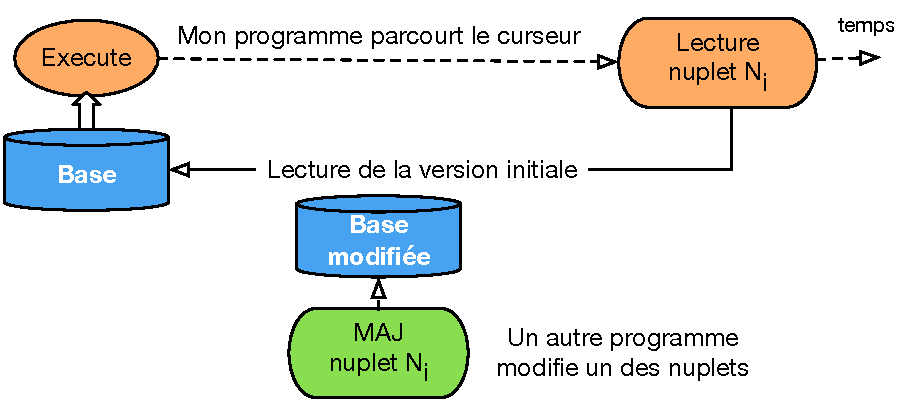
\includegraphics[width=10cm]{../figures-sql/isolation-curseur}


\vfill
Première rencontre avec la notion de \alert{concurrence} et \alert{d'isolation}.


\end{frame}

\begin{frame}[fragile]{Peut-on modifier les nuplets parcourus\,?}

Oui, avec la clause \sqlkw{current of} (si accès à une seule table)

\begin{small}
\begin{minted}{sql}
-- Déclaration du curseur
cursor CurseurLieu is select * from Lieu 

 -- Boucle for intégrant open, fetch et close
 for v_lieu in CurseurLieu loop
     update Lieu set code=UPPER(code) 
     where current of CurseurLieu;
  end loop;
\end{minted}
\end{small}

\vfill

Notez\,: ces mises à jour deviennent visibles par ma session.
\end{frame}


%%%%%%%%%%%%%
\begin{frame}{À retenir}

Les curseurs introduisent un aspect \alert{temporel} dans la gestion des données.

\vfill


Le résultat d'une requête n'est pas instantané mais exploité sur une
période de durée indéterminée.

\vfill

Soulève des questions sur la \alert{concurrence} avec d'autres sessions.

\begin{redbullet}
   \item Mes mises à jour sont-elles visibles\,?
   \item Les mises à jour des autres sessions sont-elles visibles\,?
  \item Et si on a deux mises à jour  \alert{simultanées} du même nuplet...\,?
\end{redbullet}

\vfill

Plus sur ce sujet avec la notion de \alert{transaction}.
\end{frame}
